%\chapter*{Annotation automatique d'images}
\chapter{Introduction}
Cette partie aborde les avantages ainsi que les problèmes rencontrés pour automatiser l'annotation d'images. Ensuite, notre méthodologie sera brièvement exposée pour aboutir à notre contribution.

\medskip
\section{Motivation}
\medskip

L’annotation d'images a pour but de fournir des informations textuelles à des images pour faciliter leurs exploitations. Par exemple, l'indexation d'une image est utilisée dans les systèmes textuels permettant à l'utilisateur de rechercher les images; en formulant des requêtes dans un langage naturel ou pseud naturel et exprimer ainsi ses besoins plus facilement.
%(à la différence de la recherche d'image par contenu ou CBIR).\\ 

L'annotation d'une image peut être effectuée soit par annotation textuelle manuelle, soit par annotation automatique basée sur le contenu de l'image.


L'annotation manuelle rencontre un problème sur le choix de termes utilisés pour annoter une image. L'annotateur a tendance à associer des termes qui lui semblent pertinents selon son interprétation mais qui sont souvent subjectifs et ambigus.
L'annotation manuelle est parfois effectuée par des spécialistes, les iconographes. Ces spécialistes associent les images à des mots et groupes de mots extraits d'un thesaurus ou à des catégories prédéfinies. Ce processus est très couteux en ressource humaine et temporelle compte tenu de l'immensité et la difficulté du travail à effectuer pour une grande collection d'images, même si des applications de jeux sérieux ont été développées pour palier le problème de coût financier. En alternative, l'annotation automatique est utilisée en se basant sur le contenu de l'image.\\
\qquad L'annotation automatique d'images concerne, en général, l'extraction de caractéristiques visuelles de l'image jusqu'à la prédiction des concepts sémantiques  les plus pertinents décrivant cette image (décrites par des textes). 

\medskip

\qquad On rencontre 3 types de problèmes dans l'annotation automatique d'une image selon \cite{smeulders2000content} \cite{boujemaa2004evaluation} illustrés par la Figure  \ref{fig:fausse}. Cette figure expose en parallèle la différence entre la vision humaine et un système de vision cognitive.
\medskip
\begin{figure}[h]
	\begin{center}
		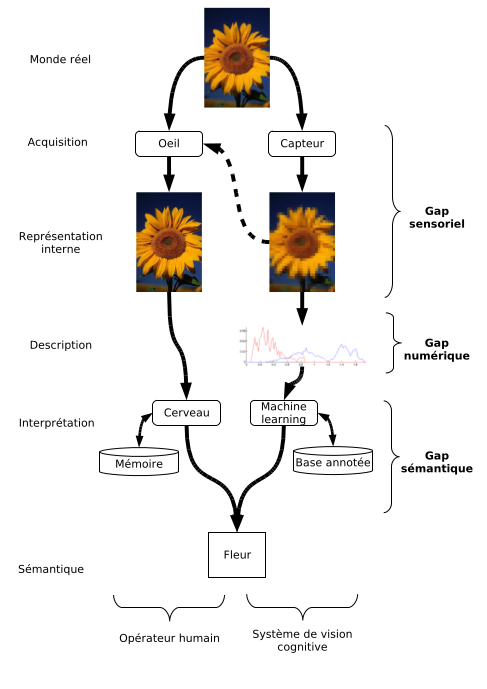
\includegraphics[width=0.7\textwidth]{fausse}
		\caption{Illustration des différents fossés \cite{herve2009vers}}
		\label{fig:fausse}
	\end{center}
\end{figure}


\smallskip
\begin{itemize}
	\item \textbf{Fossé sensoriel :} représente la perte et/ou la déformation des informations due aux appareils utilisés lors de l'acquisition de l'image numérique (appareil photo numérique, médical, satellitaire, scanner,…). 
La perte peut venir des performances de l'appareil utilisé et des bruits numériques.
%fossé
	\item \textbf{{Fossé numérique :}} \cite{herve2009vers} est la capacité d'un modèle (descripteur) à extraire les signatures visuelles pertinentes. Ce problème est lié au choix du descripteur. 
%(utilisé dans le domaine de vision par ordinateur)
 Par exemple, le choix effectué pendant le \textbf{\textit{feature engineering}} (traitement des variables) se portant sur les couleurs, la forme ou la texture, les descripteurs locaux ou globaux, cela pour extraire les caractéristiques les plus pertinentes d'une image. Dans sa thèse, Nicolas HERVE a écrit: "Le gap numérique est  l'écart entre l’information qui est présente visuellement dans une image et celle qu’un descripteur est capable d'extraire et de représenter".
% Il pose le problème de la fidélité de la signature par rapport à l’image".  
	\item \textbf{Fossé sémantique :}  problème majeure de l'annotation automatique d'images, elle peut être considérée comme le manque de corrélation entre la manière dont les humains perçoivent les informations et celle dont les ordinateurs représentent ces informations. Smeulders et al. \cite{smeulders2000content} expriment leur point de vue de le fossé sémantique: “The semantic gap is the lack of coincidence between the information that one can extract from the visual data and the interpretation that the same data have for a user in a given situation”.
A la différence de l’étude des systèmes documentaires textuels, le fossé entre les caractéristiques visuelles bas niveaux de l'image (couleur, texture,…) et ses caractéristiques sémantiques de haut niveau (description et signification) est assez large.
\end{itemize}
\qquad L'annotation automatique d'une image se résume par la modélisation de la relation entre les caractéristiques visuelles de l'image et ses caractéristiques sémantiques. D'un côté, les caractéristiques visuelles d'une image numérique peuvent être extraites par des algorithmes d'analyse d'image qui étudient la distribution des valeurs de chaque pixel de l'image. D'un autre côté, l'interprétation de cette image nous conduit à la sémantique de cette image.  Le défi majeur dans le cadre de l'annotation automatique concerne l'extraction automatique des informations sémantiques de l'image en réduisant la distance entre la signification et les caractéristiques visuelles qui correspond au fossé sémantique.\\
\smallskip
\qquad Pour réduire ce fossé sémantique, des techniques d'apprentissage automatique ont été massivement utilisées et ont abouti à de bonnes performances. A partir d’une base d’apprentissage constituée d’images déjà annotées, il est possible de construire des modèles capables par la suite de prédire des annotations pour de nouvelles images [Figure \ref{fig:apprentissage} et Figure \ref{fig:prediction}].
\medskip
\begin{figure}[h]
	\begin{center}
		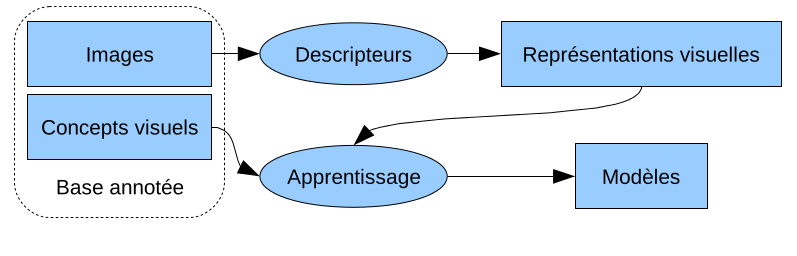
\includegraphics[width=0.7\textwidth]{apprentissage}
		\caption{Apprentissage du modèle par les données d'apprentissage \cite{herve2009vers}}
		\label{fig:apprentissage}
	\end{center}
\end{figure}
\smallskip
\begin{figure}[h]
	\begin{center}
		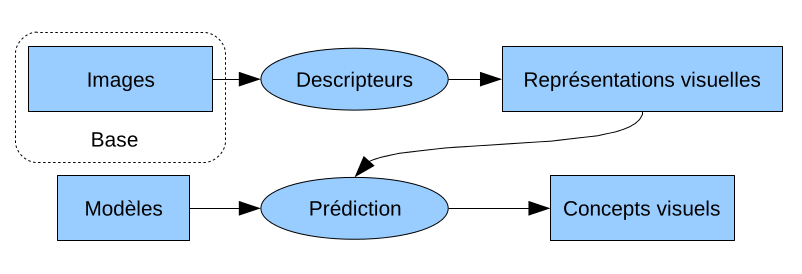
\includegraphics[width=0.7\textwidth]{prediction}
		\caption{Prédiction des concepts à partir du modèle \cite{herve2009vers}}
		\label{fig:prediction}
	\end{center}
\end{figure}
\smallskip

\medskip

\qquad Notre travail de  recherche porte sur l'étude des algorithmes d’apprentissage profond pour associer images et textes à partir des réseaux de neurones artificiels (RNA). Ces modèles très récents ont été utilisés pour représenter les images et textes afin d'extraire leur signification et ensuite les relier.\\
Nous nous sommes particulièrement intéressés à la description des images par génération de phrases descriptives ou légendes (Figure \ref{fig:phrase}). 
Les phrases \footnote{Pour reprendre la vocabulaire de la littérature du domaine, nous parlerons de "phrase" correspondant à la description d'une image, même si le texte peut ne pas respecter la grammaire de la langue} contiennent des informations plus détaillées des images. Elles sont composées de variétés de classes de mots : verbe, nom, adjectif,… qui suivent des règles grammaticales permettant de mieux décrire des images. Aussi dans les phrases, les concepts abstraits, comme \textit{riding}, sont situés dans un contexte  (\textit{people} et \textit{horse}), qui facilite leur apprentissage.
% \textbf{Exemple: "Two people riding horses side by side through a park."}
\begin{figure}[h]
	\begin{center}
		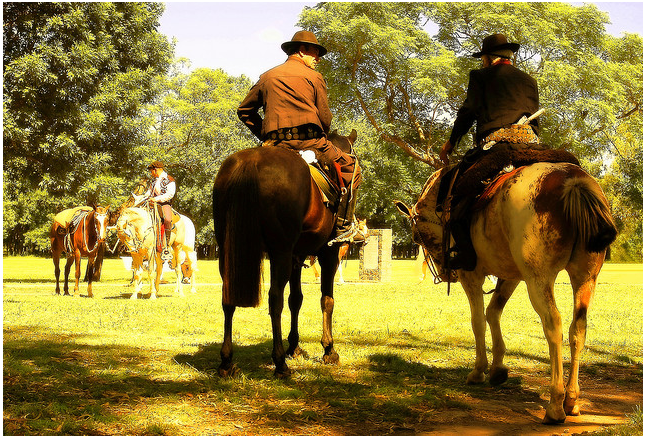
\includegraphics[width=0.4\textwidth]{cocoexamplecrop}
		 \\three men dressed like cowboys riding on horses. \\two people riding horses side by side through a park. \\a couple of men on horses in a field.
		\caption{Exemples de description d'une image par trois légendes différentes dans Microsoft COCO Captions [Chen et~al., 2015]: }
		\label{fig:phrase}
	\end{center}
\end{figure}

Une solution est d'associer directement les images et les phrases de la collection de données. Cependant, la description d'une nouvelle image nécessite des informations sur les concepts présents dans cette image pour ensuite générer de nouvelles phrases qui peuvent être différentes des phrases de cette collection. Ainsi, nous avons utilisé un modèle de génération de phrases pour la description d'une image en combinant les travaux pour la compréhension d'une image et les travaux pour la génération de phrases.

Notre proposition comprend 2 étapes: la première étape analyse les caractéristiques visuelles des images afin de les classer et la seconde fusionne les caractéristiques visuelles et textuelles pour générer des annotations.

La première étape utilise les méthodes d'apprentissage supervisé pour la classification des images. A partir des données d'apprentissage, il est possible de construire un modèle pour classifier les images dans des catégories prédéfinies. Ces catégories ou classes définissent les concepts présents dans les images.
%(objets, actions, types de lieu) 
%et  correspondent aux labels (textes associés) lors de l'annotation
 Les modèles sont créés par apprentissage de classifieurs pour grouper les images à partir de ses caractéristiques visuelles  (souvent représentés par des vecteurs) extraites des descripteurs issus des travaux dans le domaine de la vision par ordinateur comme les réseaux neuronaux convolutifs. Après avoir extrait les caractéristiques visuelles d'une nouvelle image, le modèle est utilisé pour prédire la classe correspondante. Le concept visuel associé à cette classe est ensuite attribué à cette image lors de l'annotation.
Notre étude s'est focalisée sur la classification multi-classe qui a été utilisée pour la reconnaissance de formes et d'objets \cite{krizhevsky2012imagenet}, \cite{simonyan2014very}, \cite{szegedy2015going}, \cite{sharif2014cnn}, reconnaissance de scènes \cite{zhou2014learning} dans le domaine de la vision par ordinateur.

La seconde étape de notre contribution utilise les modèles multimodaux qui exploitent la multi-modalité des données : les images et les textes associés. La tâche principale est d'analyser le contenu de l'image et de générer des descriptions textuelles en relation avec ce contenu. Les travaux effectués sont basés sur des travaux issus du domaine de la vision par ordinateur et du traitement automatique du langage naturel (TALN) pour aboutir à la génération de textes décrivant des images\cite{murthy2015automatic}, \cite{yan2015deep},\cite{fang2015captions} \cite{karpathy2015deep}.\\

\medskip
\section{Contribution}
\medskip

\qquad Inspirée de \cite{xu2015show} \cite{jia2015guiding}, notre contribution concerne l'amélioration d'un modèle de base de génération de descriptions d'images : \textit{m-RNN} : multimodal Reccurent Neural Network \cite{mao2014explain} \cite{mao2014deep} \cite{mao2015learning} en lui apportant des  informations sémantiques additionnelles sur les images. Ces informations mettent en exergue la génération de mots relatifs à l'image à décrire. L'information sémantique est définie à partir des catégories auxquelles l'image appartient et est représentée par un vecteur de scores que nous nommons : \textit{vecteur de catégories}.\\


\medskip
\section{Organisation du document}

\medskip
Le second chapitre aborde l'état de l'art de l'apprentissage profond et comporte deux sections:
\begin{itemize}
	\item La section \ref{generalite} indique les grandes lignes de l'apprentissage profond
	\item La section \ref{application}  cite les applications dans le domaine de la recherche notamment en vision par ordinateur, en traitement automatique du langage naturel  et la génération automatique de descriptions d'images.
\end{itemize}
Le troisième chapitre comporte deux sections sur notre contribution pour la génération de descriptions d'images:
\begin{itemize}
	\item La section \ref{presentationcontrib} décrit notre contribution sur un modèle de base en utilisant les résultats issus de la classification des images.
	\item La section \ref{implementation} présente les implémentations des deux parties de notre exprimentation.
\end{itemize}
Le quatrième chapitre concerne l'évaluation de notre modèle et comporte deux sections :
\begin{itemize}
	\item La section \ref{ressources} expose les ressources que nous avons utilisées lors de notre expérimentation à savoir la collection de données et les mesures d'évaluation du modèle.
	\item On retrouve dans la section \ref{resultat} les résultats obtenus. 
\end{itemize}
Le  cinquième et sixième chapitre concluent le document sur une discussion globale des méthodologies et résultats obtenus et aborde les travaux en perspective.